% These are the lecture notes for my CSCI360 course SPRING 2017
% at John Jay College of Criminal Justice.

% Feel free to edit these slides and use them for your own courses.
% HOWEVER DO NOT REMOVE THESE LINES!
% Email me at: awood [at] jjay.cuny.edu
% or at: awood [at] gradcenter.cuny.edu


\documentclass{beamer}

\usepackage{tikz}
\usetikzlibrary{calc}

\usepackage{forest}
\usepackage{verbatim}
\usepackage{color}


\setbeamertemplate{footline}[frame number]
\setbeamertemplate{navigation symbols}{} 

\newtheorem{thm}{Theorem}[section]
\newtheorem{lem}{Lemma}
\newtheorem{cl}{Claim}
\newtheorem{cor}{Corollary}[section]
\newtheorem{conj}{Conjecture}
\newtheorem{quest}{Question}
\newtheorem{defn}{Definition}[section]
\newtheorem{obs}{Observation}[section]
\newtheorem{exam}{Example}

\newcommand{\im}{\operatorname{im}}
\newcommand{\id}{\operatorname{id}}
\newcommand{\interior}{\operatorname{int}}
\newcommand{\bdry}{\operatorname{bdry}}
\newcommand{\<}{\langle}
\renewcommand{\>}{\rangle}
\newcommand{\Gab}{(G_\phi)^{ab}} 
\newcommand{\phibar}{\bar{\phi}}
\newcommand{\Z}{\mathbb{Z}}
\newcommand{\N}{\mathbb{N}}
\newcommand{\Q}{\mathbb{Q}}
\newcommand{\R}{\mathbb{R}}
\newcommand{\C}{\mathbb{C}}
\newcommand{\A}{\mathcal{A}}
\newcommand{\OO}{\mathcal{O}}
\newcommand{\UU}{\mathcal{U}}
\newcommand{\power}{2^{\{P_1, \cdots , P_n\}}}
\newcommand{\bp}{\begin{problem}}
\newcommand{\ep}{\end{problem}}
\newcommand{\ba}{\begin{answer}}
\newcommand{\ea}{\end{answer}}
\newcommand{\ds}{\displaystyle}
\newcommand{\ben}{\renewcommand{\theenumi}{\alph{enumi}}
\renewcommand{\labelenumi}{(\theenumi)}\begin{enumerate}}
\newcommand{\een}{\end{enumerate}}
\newcommand{\Hess}{\operatorname{Hessian}}
\newcommand{\Aut}{\mathrm{Aut}}
\newcommand{\Inn}{\mathrm{Inn}}
\newcommand{\Out}{\mathrm{Out}}
\newcommand{\End}{\mathrm{End}}


\mode<presentation>
{
%  \usetheme{default}
  \setbeamercovered{invisible}
}


\usepackage[english]{babel}
\usepackage[latin1]{inputenc}
\usepackage{times}
\usepackage[T1]{fontenc}
\usepackage{stmaryrd}

%\usetheme{default}
%\usetheme{AnnArbor}
%\usetheme{Antibes}
%\usetheme{Bergen}
%\usetheme{Berkeley}
%\usetheme{Berlin}
%\usetheme{Boadilla}
%\usetheme{CambridgeUS}
%\usetheme{Copenhagen}
%\usetheme{Darmstadt}
%\usetheme{Dresden}
%\usetheme{Frankfurt}
%\usetheme{Goettingen}
%\usetheme{Hannover}
%\usetheme{Ilmenau}
%\usetheme{JuanLesPins}
%\usetheme{Luebeck}
%\usetheme{Madrid}
%\usetheme{Malmoe}
%\usetheme{Marburg}
%\usetheme{Montpellier}
%\usetheme{PaloAlto}
%\usetheme{Pittsburgh}
%\usetheme{Rochester}
\usetheme{Singapore}
%\usetheme{Szeged}
%\usetheme{Warsaw}

%\usecolortheme{default}
%\usecolortheme{albatross}
\usecolortheme{beaver}
%\usecolortheme{beetle}
%\usecolortheme{crane}
%\usecolortheme{dolphin}
%\usecolortheme{dove} % grey, white, yellow
%\usecolortheme{fly} %grey, yellow
%\usecolortheme{lily} %white, yellow, blue
%\usecolortheme{orchid}
%\usecolortheme{rose}
%\usecolortheme{seagull}
%\usecolortheme{seahorse}
%\usecolortheme{whale}
%\usecolortheme{wolverine}

% Title page

\title[OOP]{Combinatorics}

\subtitle{The Mathematics of Counting}

\author
{Lecture notes of Alexander Wood \\ CSCI 360 Cryptography and Cryptanalysis \\ \scriptsize \href{mailto:awood@jjay.cuny.edu}{awood@jjay.cuny.edu}}
\institute[JJay]{John Jay College of Criminal Justice}  

\date{}

\begin{document}

% Remove 'figure' text from figure captions 
\setbeamertemplate{caption}{\raggedright\insertcaption\par}

\begin{frame}
  \titlepage
\end{frame}


\begin{frame}
\frametitle{How hard is it to count?}

Let's say you and a friend decide to flip a coin twice. How many possible heads-tails combinations are there?\newline

What if you flip it three times?
\end{frame}

\begin{frame}
\frametitle{How hard is it to count?}

\emph{What if instead of coins, you are rolling two dice? Three dice? Twenty dice?}\newline

\pause

A die has 6 sides. Thus there are six possible outcomes for the first die, and six for the second, resulting in a total of $6\times 6 = 36$ outcomes.\newline

Three dice: $6\times 6\times 6 = 6^3$ outcomes.\newline

Twenty dice: $6^{20}$ outcomes.
\end{frame}


\begin{frame}
\frametitle{HOLD UP! Exponent Review!}

\begin{itemize}
\item \textbf{Zero-Exponent Rule:} $a^0 = 1$ for any number $a$.
\item \textbf{Power Rule:} $(a^m)^n = a^{mn}$
\item \textbf{Negative Exponent Rule:} $a^{-m} = \frac{1}{a^m}$ and $\frac{1}{a^{-m}} = a^m$.
\item \textbf{Product Rule:} $a^ma^n = a^{m+n}$
\item \textbf{Quotient Rule:} $\frac{a^m}{a^n} = a^{m-n}$
\end{itemize}
\end{frame}

\begin{frame}
\frametitle{Exponents Examples}

\begin{itemize}
\item $1000^0 = 1$
\item $(4^2)^7 = 4^{14}$
\item $7^{-1} = \frac{1}{7}$
\item $\frac{1}{a^{-3}} = a^3$
\item $6^26^8 = 6^{10}$
\end{itemize}
\end{frame}

\begin{frame}
\frametitle{Exponents Examples}

\begin{align*}
2^84^6 = 2^8(2^2)^6 = 2^82^{12} = 2^{20}\\
\\
\left(\frac{x^2}{y^5}\right)^{-2} = \frac{(x^2)^{-2}}{(y^5)^{-2}} = \frac{x^{-4}}{y^{-10}} = \frac{y^{10}}{x^4}\\
\end{align*}

For more exponents examples, visit this helpful webpage:
\url{http://www.mesacc.edu/~scotz47781/mat120/notes/exponents/review/review.html}
\end{frame}



\begin{frame}
\frametitle{Counting, without counting!}

We would like to determine how many possible combinations there are given various conditions and properties. \newline

With flipping a couple coins it is easy, but what about flipping 100 coins? \newline

With some mathematics and a bit of clever thinking, we can count all sorts of things. 
\end{frame}


\begin{frame}[fragile]
\frametitle{HOLD UP! Logical Operators, aka, and vs. or}

Logical operators return Boolean (TRUE or FALSE) values.

\begin{itemize}
\item \textbf{and}: \verb|condition1 AND condition2| evaluates to True if and only if both \verb|condition1| and \verb|condition2| are true.
\item \textbf{or}: \verb|condition1 OR condition2| evaluates to True if and only if at least one of \verb|condition1| and \verb|condition2| is true.
\item \textbf{not}: \verb|NOT condition| reverses the truth value of the condition.
\end{itemize}
\end{frame}



\section{Sums \& Products}
\begin{frame}
\frametitle{The Sum Principle}

If there are $m$ ways to do $A$ and $n$ ways to do $B$, then {\color{red}the number of ways to do $A$ \textbf{or} $B$ is $m+n$}.
\end{frame}

\begin{frame}
\frametitle{The Sum Principle}

For example, say you are making dinner. There are four ways you could prepare a chicken dish, and three ways you could prepare a steak dish. \newline

How many ways could you make a chicken dish \emph{or} a steak dish? Seven.
\end{frame}

\begin{frame}
\frametitle{The Product Principle}

Say there are $m$ ways to do $A$ and $n$ ways to do $B$. {\color{red}The number of ways to do $A$ \textbf{and} $B$ is $m\times n$.} \newline

Note that here, the ways of doing $A$ and the ways of doing $B$ are \emph{independent}, meaning they do not depend on one another. (For dependent choices, see slide 7)
\end{frame}


\begin{frame}
\frametitle{Example: Subcommittees}

Say there are 5 members of your student council. How many possible ways could a subcommittee be formed?
\end{frame}

\begin{frame}
\frametitle{Solution 1: Subcommittees}

\begin{itemize}
\item There are $N1$ ways of forming 1-member subcommittees
\item There are $N2$ ways of forming 2-member subcommittees
\item There are $N3$ ways of forming 3-member subcommittees
\item There are $N4$ ways of forming 4-member subcommittees
\item There are $N5$ way(s) of forming a 5-member subcommittees
\item By the sum principle, there are
\[
N = N1+N2+N3+N4+N5
\]
ways of forming the subcommittee.
\end{itemize}
\end{frame}

\begin{frame}
\frametitle{Solution 2: Use the Product Principle}

Each student council member is either in the committee, or not in the committee. Thus it is much simpler to apply the product principle. 
\[
2 \times 2 \times 2 \times 2 \times 2= 2^5 = 32
\]
possible committee combinations.
\end{frame}


\begin{frame}
\frametitle{A bad calculation}

\begin{figure}
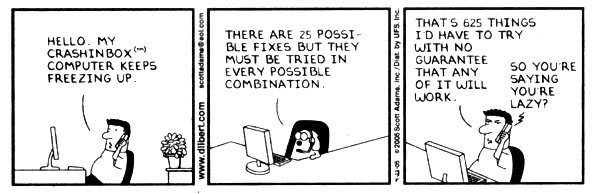
\includegraphics[scale=.5]{IMG/comic.jpg}
\end{figure}

The math here is incorrect. How many things would they actually need to try?
\end{frame}


\begin{frame}
\frametitle{Combinatorics and Security: PINs}

Each digit in your PIN can be one of 10 values (0, 1, 2, $\dots$, 9). Your PIN is four numbers long. How many possible PIN numbers are there?\newline

\pause

There are 10 choices for each value, so there are
\[
10 \times 10 \times 10 \times 10 = 10^4 = 10,000
\]
possible PIN choices.
\end{frame}

\begin{frame}
\frametitle{Combinatorics and Security: PINs}

Say you are trying to break into someone's bank account. You can try one PIN every 5 seconds. How long would it take to check every combination? \newline

\pause

Solution:
\[
10,000 \text{ combinations} \times 5 \text{ seconds } = 50,000 \text{ seconds}
\]
or 13 hours, 53 minutes, and 20 seconds. 
\end{frame}

\begin{frame}
\frametitle{Combinatorics and Security: PINs}

Say that you are only able to try entering the PIN 10 times before the system locks you out. What is your probability of success?\newline\pause

You can try 10 out of 10,000 possible combinations, so your probability of success is 
\[
\frac{10}{10,000} = \frac{1}{1,000} = 0.001 = 0.1\%
\]
\end{frame}


\section{Permutations}


\begin{frame}
\frametitle{How hard is it to count?}

\emph{You'd like to visit all 5 boroughs of NYC. How many different ways can you do this?}
\newline

\pause

There are $5$ ways to pick the first borough, $4$ ways to pick the second, $3$ ways to pick the third, $2$ ways to pick the fourth, and $1$ way to pick the last. Thus there are
\[
5! = 5 \times 4 \times 3 \times 2 \times 1
\]

\end{frame}


\begin{frame}
\frametitle{HOLD UP! What's a factorial?!}

Factorials are just products. For a positive integer $n$ define
\[
n! = n(n-1)(n-2)\cdots(2)(1)
\]

Examples:
\begin{itemize}
\item $4! = 4(3)(2)(1) = 24$
\item $6! = 6(5)(4)(3)(2)(1) = 720$
\end{itemize}
\end{frame}


\begin{frame}
\frametitle{Permutations Example}

Sarah, Juan, and Belle take a cab to the movies and sit in the back seat. How many possible ways are there that they can sit in the back of the cab?\newline

\pause

There are three choices for who sits on the left, two choices for who sits in the middle, and one remaining choice for who sits on the right. Thus there are
\[
3! = 3\times 2 \times 1 = 6
\]
ways for them to arrange themselves in the back seat.
\end{frame}

\begin{frame}
\frametitle{Permutations}

A \textbf{permutation}, or an \textbf{ordering}, is the number of ways of arranging items in some order. {\color{red}The number of permutations of $n$ objects is given by $n!$.}
\end{frame}

\begin{frame}
\frametitle{Even more permutations}

We have five letters, (A, B, C, D, E), and we wish to find all possible permutations of three of these letters. For example, ABC, CBA, ABD, CDE, EBC, etc. \newline

\pause

There are five choices for the first letter, four choices for the second letter, and three choices for the second letter.
\[
5\times 4 \times 3 = 60 \text{ choices}
\]
\end{frame}


\begin{frame}
\frametitle{Permutations}

The {\color{red}number of permutations of $n$ objects taken $k$ at a time} is given by
\[
\frac{n!}{(n-r)!} = n(n-1)\cdots(n-r+1)
\]
\end{frame}

\begin{frame}
\frametitle{Permutations \& Security}

You decide to disguise a message by replacing each of 26 English letters with a letter from a Chinese character dictionary you own, picking from the 50 most frequently-used characters.  How many possible ways could you set up your cipher?\newline 

\pause

This is a permutation problem! We want to know how many possible ways we can associate each letter in the English language with one of 30 Chinese characters. In other words, how many permutations of these 30 characters are there, taken 26 at a time?
\[
\frac{30!}{(30-26)!} = \frac{30!}{4!} = 11052202492174627443179520000000
\]
\end{frame}

\section{Combinations} 

\begin{frame}
\frametitle{Combinations Example}

How many ways are there to choose 4 letters out of 7 letters? \newline

\pause

There are $\frac{7!}{(7-4)!} = 840$ permutations of 4 letters taken from 7 letters. However, now we need to discard all permutations, since ABCD, DCBA, BADC, etc, are all the same case now. \newline

\pause

Note that each four-letter choice has $4!$ permutations. Thus the total number of ways to choose four letters out of seven letters is 
\[
\frac{7!}{4!(7-4)!} = 35
\]
\end{frame}




\begin{frame}
\frametitle{Combinations}

The {\color{red}number of possible ways of picking $k$ (unordered) outcomes from $n$ possibilities} is called the number of \textbf{combinations}, or the \textbf{binomial coefficient}. It is denoted by $n\choose k$, pronounced ``n choose k,'' and given by 
\[
{n \choose k} = \frac{n!}{k!(n-k)!}
\]
\end{frame}


\section{Class Exercises}


\begin{frame}
\frametitle{Exercise 1}

A door lock has a key pad with the numbers 1 through 9. The key to the door consists of a sequence of six digits. How many possible keys are there?
\end{frame}

\begin{frame}
\frametitle{Solution 1}

There are $9^6$ possible keys.
\end{frame}

\begin{frame}
\frametitle{Exercise 2}

A gym lock dial has 50 numbers, and you unlock it by turning the dial 3 times to 3 numbers. If a thief can check 6 combinations per minute, how long will it take the thief to check all possible combinations?
\end{frame}

\begin{frame}
\frametitle{Solution 2}

There are $50^3$ possible lock combinations. At a rate of 6 per minute, it will take the theif 
\[
\frac{50^3}{6} = 20833.\bar{3} \text{ minutes}
\]
or 14 days, 11 hours, 13 minutes, and 20 seconds.
\end{frame}

\begin{frame}
\frametitle{Exercise 3}

A nuclear missile launcher requires 6 physical keys to be activated. These 6 keys are stored in a box with 30 other decoy keys. If someone was to grab 6 keys from this cabinet, what is the likelihood that they could launch the missile?
\end{frame}

\begin{frame}
\frametitle{Solution 3}

The order in which we pick the keys does not matter, as long as we pick all 6 of the correct keys. Thus we first wish to deduce how many possible ways there are to choose 6 keys out of 36 keys (decoy keys plus real keys). This is given by
\[
{36 \choose 6} = 1,947,792 \text{ possibilities}
\]
\end{frame}

\begin{frame}
\frametitle{Solution 3 cont.}

Only one of these possible ways of grabbing the keys is correct, so the probability of randomly grabbing the correct key combo is given by
\[
\frac{1}{1947792} \approx 5.13 \times 10^{-7} = 0.0000513 \%
\]
\end{frame}


\begin{frame}
\frametitle{Quiz Next Week!}

Some sample problems will be posted on the course Piazza page. You can use the Piazza platform to discuss any problems you get stuck on with your classmates and myself.
\end{frame}

\begin{frame}
\frametitle{References and Further Reading}

\begin{itemize}
\item \url{http://www.cs.cornell.edu/courses/cs280/2004fa/280wk6_x4.pdf}
\end{itemize}
\end{frame}
\end{document}


